\documentclass[paper=a4, fontsize=11pt]{scrartcl}
\usepackage[T1]{fontenc}
\usepackage{fourier}

\usepackage[english]{babel}															% English language/hyphenation
\usepackage[protrusion=true,expansion=true]{microtype}	
\usepackage{amsmath,amsfonts,amsthm} % Math packages
\usepackage[pdftex]{graphicx}	
\usepackage{url}


%%% Custom sectioning
\usepackage{sectsty}
\allsectionsfont{\centering \normalfont\scshape}
\usepackage{subfigure}


%%% Custom headers/footers (fancyhdr package)
\usepackage{fancyhdr}
\pagestyle{fancyplain}
\fancyhead{}											% No page header
\fancyfoot[L]{}											% Empty 
\fancyfoot[C]{}											% Empty
\fancyfoot[R]{\thepage}									% Pagenumbering
\renewcommand{\headrulewidth}{0pt}			% Remove header underlines
\renewcommand{\footrulewidth}{0pt}				% Remove footer underlines
\setlength{\headheight}{13.6pt}


%%% Equation and float numbering
\numberwithin{equation}{section}		% Equationnumbering: section.eq#
\numberwithin{figure}{section}			% Figurenumbering: section.fig#
\numberwithin{table}{section}				% Tablenumbering: section.tab#


%%% Maketitle metadata
\newcommand{\horrule}[1]{\rule{\linewidth}{#1}} 	% Horizontal rule

\title{
		%\vspace{-1in} 	
		\usefont{OT1}{bch}{b}{n}
		\normalfont \normalsize \textsc{CS650 - Computer Vision} \\ [25pt]
		\horrule{0.5pt} \\[0.4cm]
		\huge Programming Lab 1 - Image Processing \\
		\horrule{2pt} \\[0.5cm]
}
\author{
		\normalfont 								\normalsize
        Daqing Yi\\[-3pt]		\normalsize
        \today
}
\date{}


%%% Begin document
\begin{document}
\maketitle

Prepare a brief (but specific and well-articulated) write-up about your methods, observations, and conclusions.
Include some images to illustrate your results (you may need to crop and zoom so we can see detail - we do not necessarily need entire images or all results, but enough to be representative of what you have done and demonstrate what you are writing about).

\begin{itemize}
\item What do you conclude about binarization? 
\item What do you conclude about the use of morphological open and close operations?
\end{itemize}

There are no specific right or wrong answers--do your best to think about the methods, their strengths, and their weaknesses.

\section{Binarization}

Otsu's method finds a threshold that separates the pixels into foreground class and background class.
The objective is defined as minimizing the intra-class variance $ \omega_{f} (t) \sigma_{f}^{2} (t) + \omega_{b} (t) \sigma_{b}^{2} (t) $, which equals to maximizing inter-class variance $ \omega_{f} (t) \omega_{b} (t) [ \mu_{f} (t) - \mu_{b} (t) ]^{2} $.
$ t \in [1, N] $ is the intensity level.
$ \omega_{f} (t) $ and $ \omega_{b} (t) $ are the weights of two classes, which are calculated from histogram $ \sum_{i=1}^{t} p(i) $ and $ \sum_{i=t+1}^{N} p(i) $.
$ \mu_{f} (t) $ and $ \mu_{b} (t) $ are the means of two classes, which are computed from $ \sum_{i=1}^{t} i * p(i) $ and $ \sum_{i=t+1}^{N} i * p(i) $.

\begin{figure}
\centering
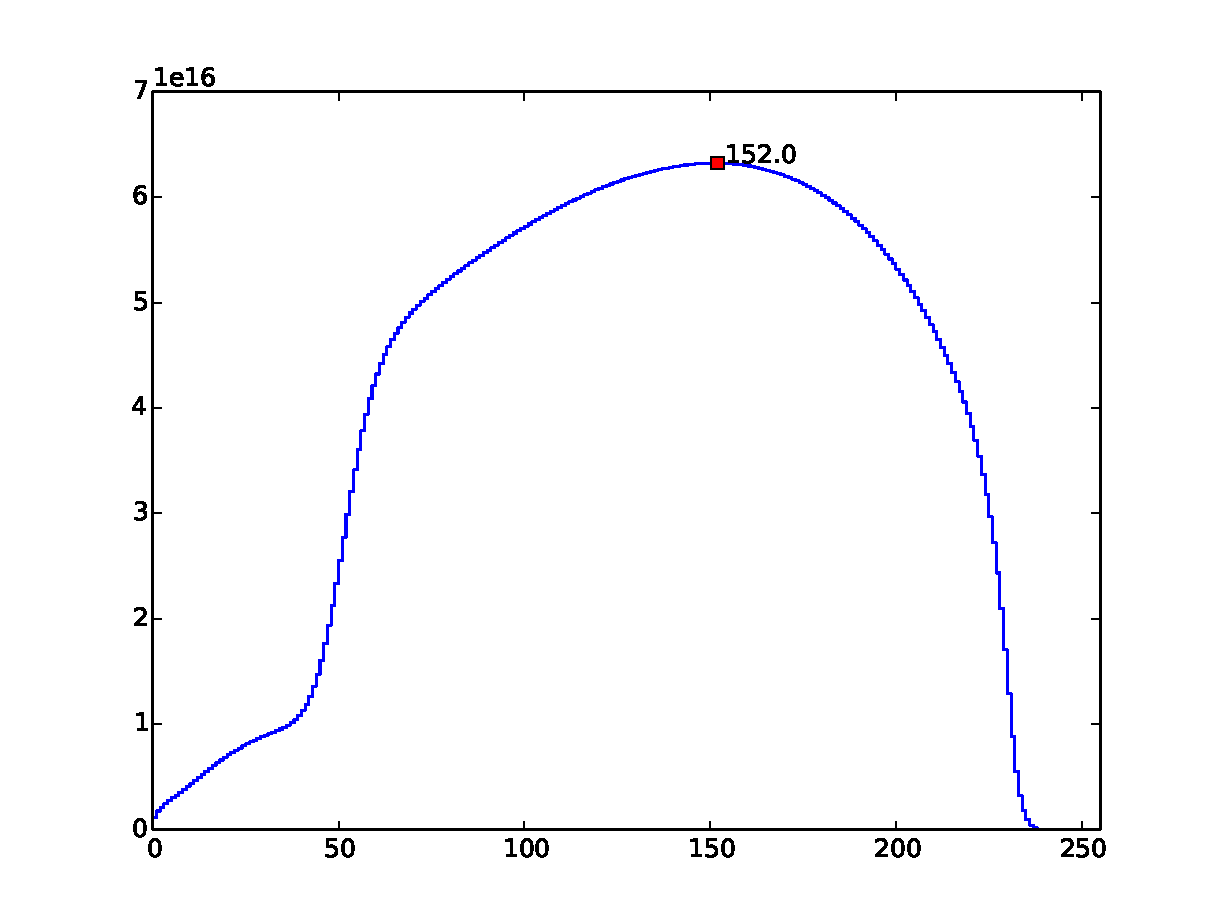
\includegraphics[width=0.6\linewidth]{./figure/interclass_variances}
\caption{Finding the maximum interclass variance}
\label{fig:interclass_variances}
\end{figure}

Otsu's method uses an exhaustive search to find the optimal solution, like in Figure \ref{fig:interclass_variances}. 

\subsection{Implementation}

The functions are written in \emph{binarization.py}.

\begin{itemize}
\item \textbf{ otsu(hist, total) } reads the histogram and total number of the pixels, then returns the threshold.
\item \textbf{ binarize(img\_data, threshold, on\_value=1) } converts the image data array into binary data array by threshold.
On\_value indicates the number stored for representing ON pixel.
\end{itemize}

\subsection{Results}

\subsubsection{0397.pgm}

\begin{figure}
\centering
\subfigure[Origin]{
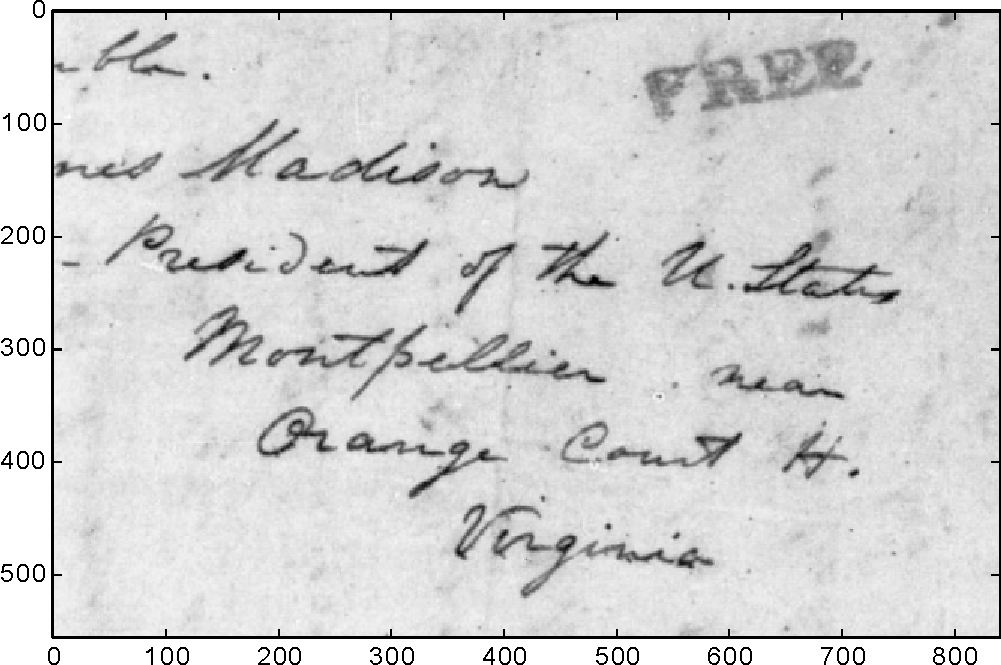
\includegraphics[width=.45\textwidth]{./figure/0397_pgm_origin}
\label{fig:binary:01:origin} }
\subfigure[Binary]{
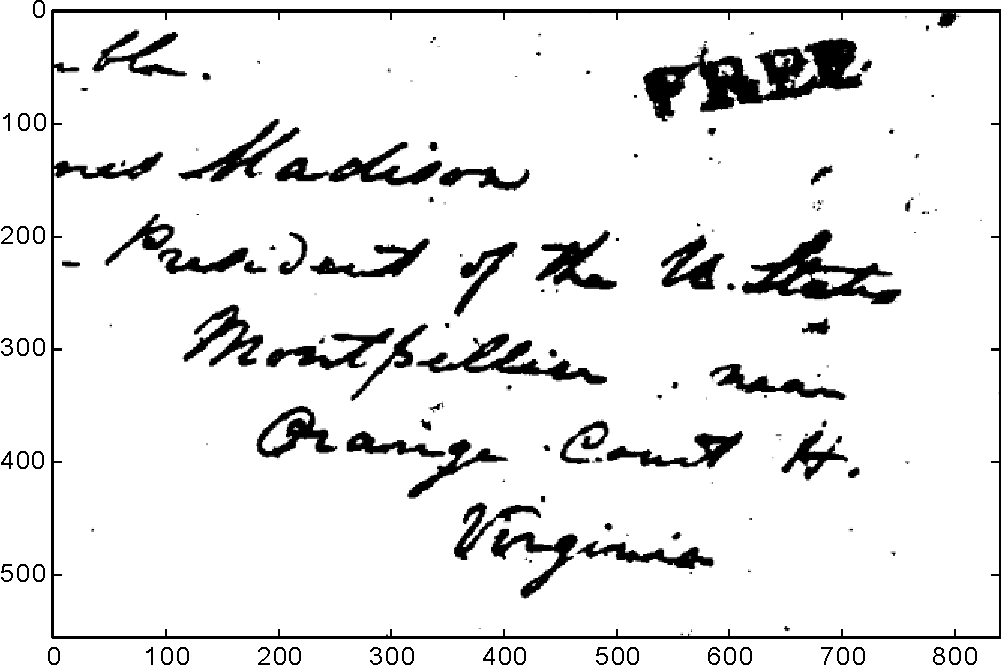
\includegraphics[width=.45\textwidth]{./figure/0397_pgm_binary}
\label{fig:binary:01:binary} }
\caption{Binarization of 0397.pgm using Otsu's method.}\label{fig:binary:01}
\end{figure}

\subsubsection{other cases}

\begin{table}
\label{tab:title}
\caption {Comparison on the results of \textbf{threshold} obtained from different implementations of Otsu's method.}
\begin{center}
\begin{tabular}{ | l | l | l | }
\hline
test file & Threshold (My code) & Threshold (Open CV)  \\ \hline
0397.pgm                                          & 134 & 134 \\ \hline
020206\_131612\_bp001\_folio\_094\_k639\_1837.ppm & 182 & 182 \\ \hline
Declaration\_Pg1of1\_AC\_crop.pgm                 & 186 & 186 \\ \hline
Scan\_half\_crop\_norm\_009\_small.pgm            & 134 & 134 \\ \hline
seq-4\_small.pgm                                  & 152 & 152 \\ \hline
\end{tabular}
\end{center}
\end{table}


\section{Morphology}



\subsection{Implementation}

The functions are written in \emph{morphology.py}.

\begin{itemize}
\item \textbf{ countNum( img\_data, maskSize ) } xcxx
\item \textbf{ dataThreshold( data, threshold, ratio=1.0 ) }  xxx
\end{itemize}

There is also a class \emph{NorphologicalFiltering}.
It stores the \emph{maskSizeData} used for operations \textbf{dilate}, \textbf{erode}, \textbf{open} and \textbf{close}.


\subsection{Results}

\subsubsection{Letter J}

\begin{figure}
\centering
\subfigure[Binary]{
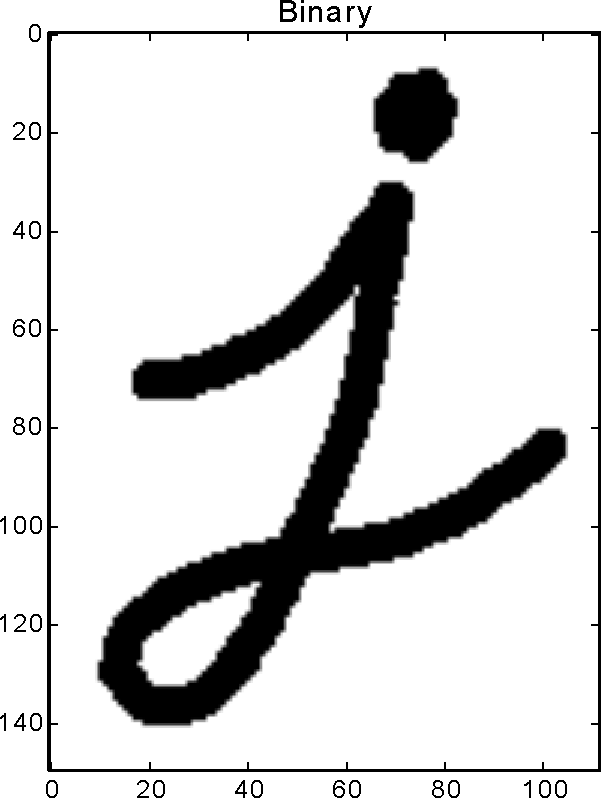
\includegraphics[width=.3\textwidth]{./figure/J_binary}
\label{fig:j_binary} }
\subfigure[Dilate]{
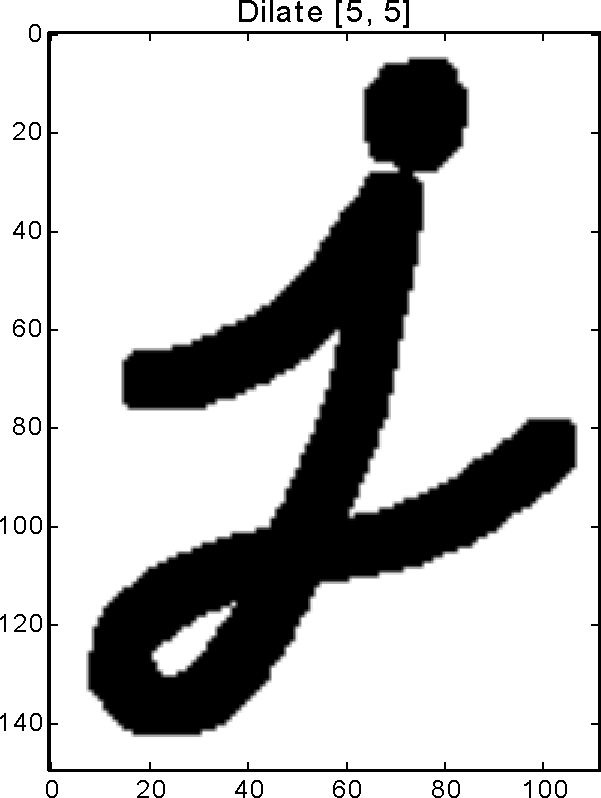
\includegraphics[width=.3\textwidth]{./figure/J_dilate}
\label{fig:j_dilate} }
\subfigure[Erode]{
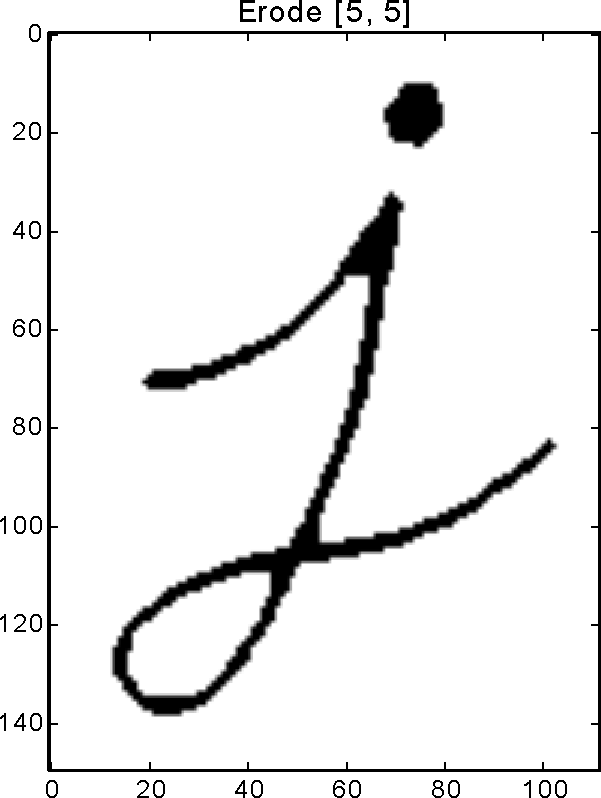
\includegraphics[width=.3\textwidth]{./figure/J_erode}
\label{fig:j_erode} }
\subfigure[Open]{
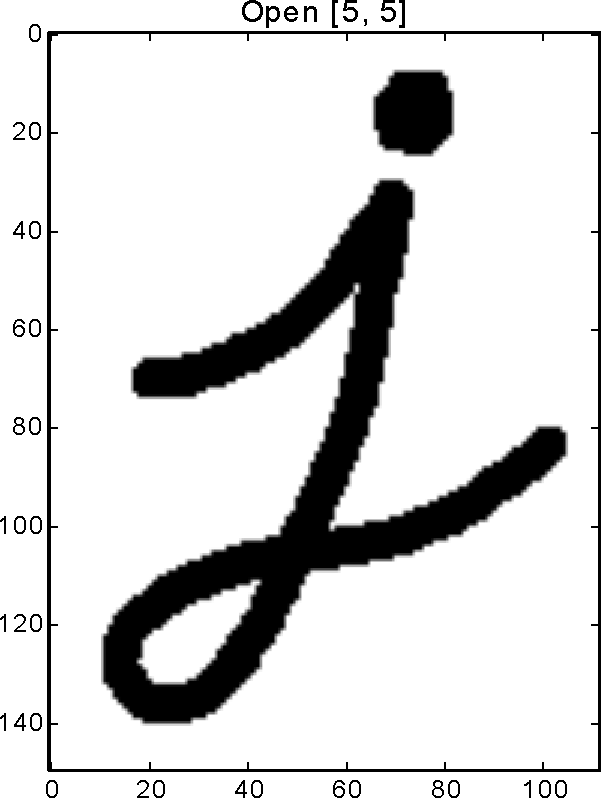
\includegraphics[width=.3\textwidth]{./figure/J_open}
\label{fig:j_open} }
\subfigure[Close]{
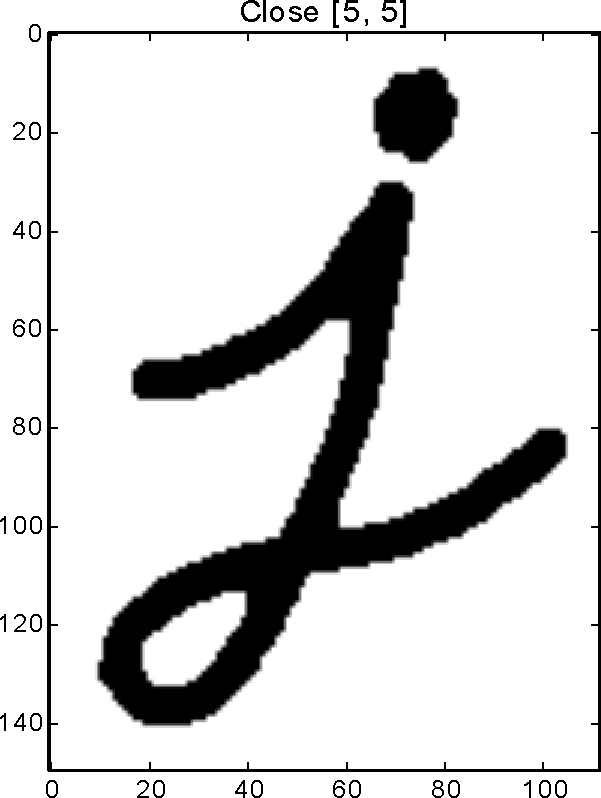
\includegraphics[width=.3\textwidth]{./figure/J_close}
\label{fig:j_close} }
\caption{Morphology operations of Letter J.}\label{fig:j_letter}
\end{figure}

\subsubsection{Yihi}

\end{document}